\documentclass[a4paper]{article}
\usepackage{graphicx}  
\usepackage[landscape]{geometry}
\usepackage[dvipdfm]{color}

\usepackage{quickrefcard}

\usepackage{multicol}
\usepackage{amsmath}
\usepackage{amsfonts}

\begin{document}
\begin{multicols*}{3}
\begin{center}
\textbf{Sage Quick Reference: Calculus}\\
William Stein (modified by nu)\\
Sage Version 3.4\\
\url{http://wiki.sagemath.org/quickref}\\
GNU Free Document License, extend for your own use
\end{center}
\vspace{-2ex}

%*********************************************
\sect{Builtin constants and functions}

Constants: 
      $\pi$=\EX{pi}
\quad    $e$=\EX{e} 
\quad    $i$=\EX{I}=\EX{i}
\BreakLineAndIndent
    $\infty$=\EX{oo}=\EX{infinity} 
\quad
    NaN=\EX{NaN} 
\quad    $\log(2)$=\EX{log2}
\BreakLineAndIndent
    $\phi$=\EX{golden_ratio} 
\quad    $\gamma$=\EX{euler_gamma}
\BreakLineAndIndent
      0.915$\approx$\EX{catalan}
\quad 2.685$\approx$\EX{khinchin}
\quad 0.660$\approx$\EX{twinprime}
\BreakLineAndIndent
 0.261$\approx$\EX{merten}
\quad 1.902$\approx$\EX{brun}

Approximate: 
\EX{pi.n(digits=18)} $=3.14159265358979324$

Builtin functions: 
\sagecommand{sin} 
\sagecommand{cos} 
\sagecommand{tan} 
\sagecommand{sec} 
\sagecommand{csc} 
\sagecommand{cot} 
\sagecommand{sinh} 
\sagecommand{cosh} 
\sagecommand{tanh} 
\sagecommand{sech} 
\sagecommand{csch} 
\sagecommand{coth} 
\sagecommand{log} 
\sagecommand{ln} 
\sagecommand{exp} \ldots

%*********************************************
\sect{Defining symbolic expressions}

Create symbolic variables:
\BreakLineAndIndent
\EX{var("t u theta")} or \EX{var("t,u,theta")}

Use \sagecommand{*} for multiplication and \sagecommand{^} for exponentiation:
\BreakLineAndIndent
$ 2x^5 + \sqrt{2} = $\EX{2*x^5 + sqrt(2)}

Typeset: \EX{show(2*theta^5 + sqrt(2))} $ \longrightarrow 2\theta^5 + \sqrt{2}$

%*********************************************
\sect{Symbolic functions}

Symbolic function (can integrate, differentiate, etc.):  
\BreakLineAndIndent
\EX{f(a,b,theta) = a + b*theta^2}

Also, a ``formal'' function of theta:
\BreakLineAndIndent
\EX{f = function('f',theta)}

Piecewise symbolic functions:\\
\EX{Piecewise([[(0,pi/2),sin(1/x)],[(pi/2,pi),x^2+1]])}

%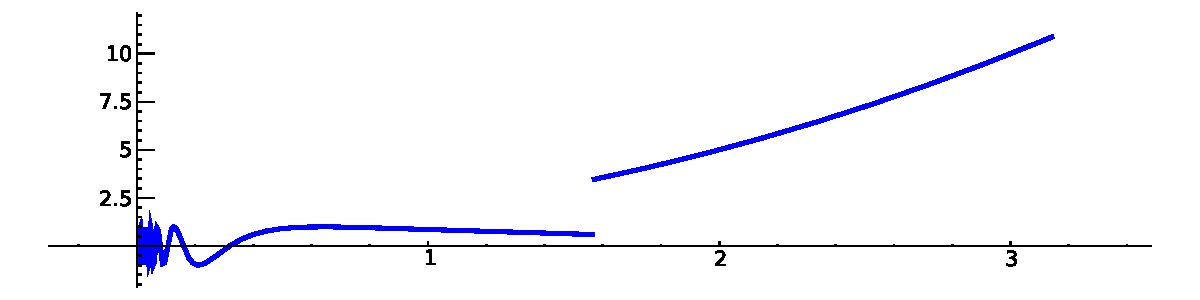
\includegraphics[width=25em]{piecewise.pdf}
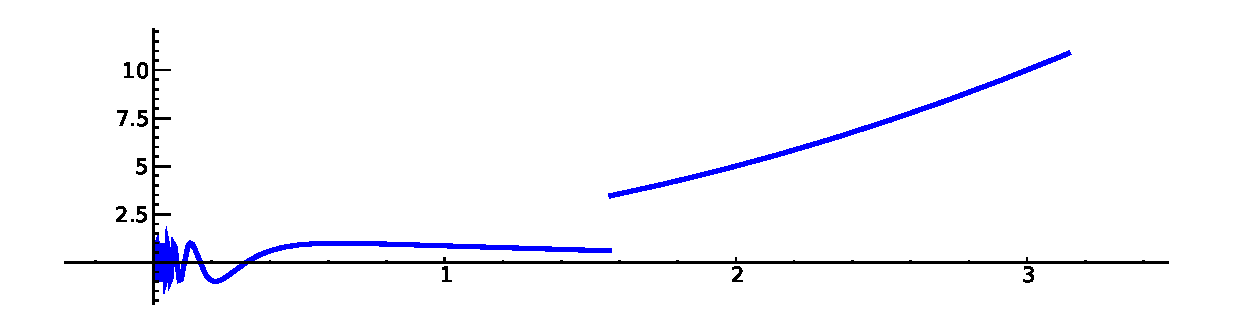
\includegraphics[width=25em]{piecewise.eps}

%*********************************************
 \sect{Python functions}

Defining:                           \BreakLineAndIndent
{\ex
\verb|def f(a, b, theta=1):|    \BreakLineAndIndent
\verb|    c = a + b*theta^2|       \BreakLineAndIndent
\verb|    return c|}

Inline functions:
\BreakLineAndIndent
\EX{f = lambda a, b, theta = 1: a + b*theta^2}

%*********************************************
\sect{Simplifying and expanding}

Below $f$ must be symbolic (so {\bf not} a Python function):

Simplify: 
\sagecommand{f.simplify_exp()}      \@
\sagecommand{f.simplify_full()}     \@
\BreakLineAndIndent[\phantom{Simplify:}]
\sagecommand{f.simplify_log()}      \@
\sagecommand{f.simplify_radical()}  \@
\BreakLineAndIndent[\phantom{Simplify:}]
\sagecommand{f.simplify_rational()} \@
\sagecommand{f.simplify_trig()}     \@

Expand: 
\sagecommand{f.expand()} \@ 
\sagecommand{f.expand_rational()}


%*********************************************
\sect{Equations}

Relations: 
$f=g$: \sagecommand{f == g},      \hfil
$f\neq g$: \sagecommand{f != g}, 
\BreakLineAndIndent[\phantom{Relations:}]
$f\leq g$: \sagecommandtt{f <= g},         \hfil
$f\geq g$: \sagecommandtt{f >= g}, 
\BreakLineAndIndent[\phantom{Relations:}]
$f< g$:    \sagecommandtt{f < g},          \hfil
$f> g$:    \sagecommandtt{f > g} 

Solve $f=g$: \sagecommand{solve(f == g, x)}, and
\BreakLineAndIndent[\phantom{Solve $f=g$:}]
\sagecommand{solve([f == 0, g == 0], x,y)}
\BreakLineAndIndent
\EX{solve([x^2+y^2==1, (x-1)^2+y^2==1],x,y)}

Solutions: 
\BreakLineAndIndent
\EX{S = solve(x^2+x+1==0, x, solution_dict=True)}
\BreakLineAndIndent
\EX{S[0]["x"]   S[1]["x"]} are the solutions

Exact roots: \EX{(x^3+2*x+1).roots(x)}\\
Real roots: \EX{(x^3+2*x+1).roots(x,ring=RR)}\\
Complex roots: \EX{(x^3+2*x+1).roots(x,ring=CC)}

%*********************************************
\sect{Factorization}

Factored form: \EX{(x^3-y^3).factor()}\\
List of (factor, exponent) pairs:
\EX{(x^3-y^3).factor_list()}

%*********************************************
\sect{Limits}

$\displaystyle\lim_{x\to a} f(x)=$ \sagecommand{limit(f(x), x=a)}
\BreakLineAndIndent
\EX{limit(sin(x)/x, x=0)}

$\displaystyle\lim_{x\to a^+} f(x)=$ \sagecommand{limit(f(x), x=a, dir='plus')}
\BreakLineAndIndent
\EX{limit(1/x, x=0, dir='plus')}

$\displaystyle\lim_{x\to a^-} f(x)=$ \sagecommand{limit(f(x), x=a, dir='minus')}
\BreakLineAndIndent
\EX{limit(1/x, x=0, dir='minus')}



%*********************************************
\sect{Derivatives}

$\frac{d}{dx}(f(x))=$ \sagecommand{diff(f(x),x) = f.diff(x)}

$\frac{\partial}{\partial x}(f(x,y))=$ \sagecommand{diff(f(x,y),x)}

\sagecommand{diff} $=$ \sagecommand{differentiate} $=$ \sagecommand{derivative}
\BreakLineAndIndent
\EX{diff(x*y + sin(x^2) + e^(-x), x)}


%*********************************************
\sect{Integrals}

$\int f(x)dx=$ \sagecommand{integral(f,x) = f.integrate(x)}
\BreakLineAndIndent
\EX{integral(x*cos(x^2), x)}

$\int_a^b f(x)dx=$ \sagecommand{integral(f,x,a,b)}
\BreakLineAndIndent
\EX{integral(x*cos(x^2), x, 0, sqrt(pi))}

$\int_a^b f(x)dx \approx$ \sagecommand{numerical_integral(f(x),a,b)[0]}
\BreakLineAndIndent
\EX{numerical_integral(x*cos(x^2),0,1)[0]}

\sagecommand{assume(...)}: use if integration asks a question
\BreakLineAndIndent
\EXtt{assume(x>0)}

%\mbox{}\,\quad([0] gives integral and [1] gives error bound)

%*********************************************
\sect{Taylor and partial fraction expansion}

Taylor polynomial, deg $n$ about $a$:\\
\sagecommand{taylor(f,x,a,n)}$\approx c_0 + c_1(x-a) + \cdots + c_n(x-a)^n$
\BreakLineAndIndent
\EX{taylor(sqrt(x+1), x, 0, 5)}

Partial fraction:
\EX{(x^2/(x+1)^3).partial_fraction()}


%*********************************************
\sect{Numerical roots and optimization}

Numerical root: \sagecommand{f.find_root(a, b, x)}
\BreakLineAndIndent
\EX{(x^2 - 2).find_root(1,2,x)}

Maximize: find $(m,x_0)$ with $f(x_0)=m$ maximal
\BreakLineAndIndent
\sagecommand{f.find_maximum_on_interval(a, b, x)}

Minimize: find $(m,x_0)$ with $f(x_0)=m$ minimal
\BreakLineAndIndent
\sagecommand{f.find_minimum_on_interval(a, b, x)}

Minimization: \sagecommand{minimize(f,}\sagevar{start_point}\sagecommand{)}
\BreakLineAndIndent
\EX{minimize(x^2+x*y^3+(1-z)^2-1, [1,1,1])}

%*********************************************
\sect{Multivariable calculus}

Gradient: \sagecommand{f.gradient()} or \sagecommand{f.gradient(}\sagevar{vars}\sagecommand{)}
\BreakLineAndIndent
\EX{(x^2+y^2).gradient([x,y])}

Hessian: \sagecommand{f.hessian()}
\BreakLineAndIndent
\EX{(x^2+y^2).hessian()}

Jacobian matrix: \sagecommand{jacobian(f,}\sagevar{vars}\sagecommand{)}
\BreakLineAndIndent
\EX{jacobian(x^2 - 2*x*y, (x,y))}

%*********************************************
\sect{Summing infinite series}

$$\sum_{n=1}^{\infty} \frac{1}{n^2} = \frac{\pi^2}{6}$$

{\em Not yet implemented, but you can use Maxima:}
\BreakLineAndIndent
\EX{s = 'sum (1/n^2,n,1,inf), simpsum'}
\BreakLineAndIndent
\EX{SR(sage.calculus.calculus.maxima(s))}
$\longrightarrow \pi^2/6$



\end{multicols*}

\end{document}
